\documentclass{article}
\usepackage{graphicx} % Required for inserting images

\title{Ultrahangos mérés}
\author{Kern Luca, Csongor Vincze}
\date{2026 Február 25}

\begin{document}

\maketitle

\section{1. Feladat Ismerkedés az oszcilloszkóp és a függvénygenerátor használatával.}

Beállítottuk a 4 V amplitúdójú, 1 V eltolású 115 Hz-es szinuszjelet. Csatlakoztattuk a jelet az oszcilloszkóphoz is. Beállítottuk a triggert, és stabilizáltuk, ízlésesen a képernyő közepér hoztuk a jelet.
Végül közelítőleg lemértük a jel amplitúdóját és frekvenciáját.

\begin{table}[h!]
    \centering
    \begin{tabular}{|l|c|c|c|}
        \hline
        Paraméter & Beállított érték & kurzorral mért érték & funkcióval mért érték \\ \hline
        Amplitúdó 4,0 ?? & 4,0 & 4,0 \\ \hline
        Frekvencia 115,0 & 116,3 & 114,9 \\ \hline
    \end{tabular}
    \caption{A beállított és a mért amplitúdó és frekvencia értékek.}
    \label{tab:amplitudo_frekvencia}
\end{table}

A különbség az RMS és a csúcstól csúcsig mért értékek között a fő különbség, hogy a csúcstól csúcsig mért érték az amplitúdó kétszerese, míg az effektív érték a jel négyzetének a kiátlagolásának a gyöke.

Megváltoztattuk a csatolási módot DC-ről AC-re, így kiküszöböltük a konstans tagú feszültség miatti eltolást.
Ha a csatolást "Ground"-ra állítottuk a következő történt:

Végül a kurzor egyenesek segítségével is megmértük az amplitúdó és frekvencia értékeit a jelnek.


\begin{figure}[htp]
    \centering
    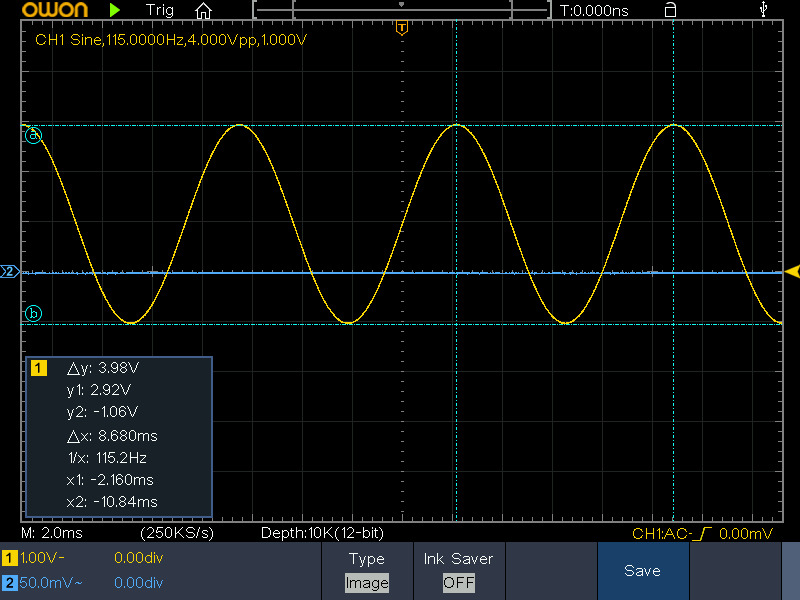
\includegraphics[width=4cm]{1.42.jpg}
    \caption{Az oszcilloszkóp különböző funkcióinak kipróbálása}
    \label{probalkozas}
\end{figure}

\section{Ultrahangos adó-vevő páros átviteli karakterisztikája
a frekvencia függvényében}

Lehelyeztük a két adó-vevőt körülbelül 10 cm távolságra, és kissé elforgattuk őket, hogy ne zavarjanak be a visszaverődő hullámok. Ezután beállítottuk az 6 V-os eltolásmentes színuszjelet. Csatlakoztattuk az koax kábelt a jelgenerátorhoz, aztán egy koaxkábeles elosztóval bekötöttük a jelet az oszcilloszkópba és az adóba is. Az oszcilloszkóp másik bemenetéhez pedig csatlakoztattuk a vevőt. Ezután beállítottuk a triggert.

\begin{table}[h!]
    \centering
    \begin{tabular}{|c|c|}
        \hline
        Frekvencia [kHz] & Amplitúdó [mV] \\ \hline
        1 & 10.0 \\ \hline 
        5 & 11.0\\ \hline
        10 & 10.0\\ \hline 
        15 & 10.5\\ \hline
        20 & 9.5\\ \hline
        25 & 10.0\\ \hline
        30 & 9.5\\ \hline
        35 & 11.0\\ \hline
        40 & 174.0\\ \hline
        45 & 12\\ \hline
        50 & 11.5\\ \hline
        55 & 10.5\\ \hline
        60 & 10.0\\ \hline
        65 & 11.5\\ \hline
        70 & 10.0\\ \hline
        75 & 11.0\\ \hline
        80 & 10.5\\ \hline
        85 & 9.5\\ \hline
        90 & 9.5\\ \hline
        95 & 10.5\\ \hline
        100 & 9.5\\ \hline
    \end{tabular}
    \caption{Az adó-vevő páros átviteli karakterisztikájának mérési adatai.}
    \label{tab:atviteli_karakterisztika}
\end{table}


\begin{enumerate}
    \item A legalacsonyabb frekvenciájú jel, amit ezzel a beállítással mérni lehet: 
    \item A frekvencia, amitől kezdve hallani kezdjük a jelet: 5kHz
    \item A legmagasabb frekvencia, amit még hallunk: 17,4kHz
    \item A rezonanciafrekvenciák: 40,27 kHz (itt 179,1 mV ampilitúdót mértünk), 51,9 kHz (itt 19 mV  volt), 93,5 kHz (itt 2,6 mV volt a mért adat)
    \item A rezonanciafrekvencia, amely a legnagyobb csúcsot adja: 40,27 kHz, itt a csúcs 179,1 mV volt
\end{enumerate}


\begin{table}[h!]
    \centering
    \begin{tabular}{|c|c|}
        \hline
        Frekvencia [kHz] & Amplitúdó [mV] \\ \hline
        38,0 & 35.0 \\ \hline
        39,0 & 70.0 \\ \hline
        39,2 & 78.5 \\ \hline
        39,4 & 98.0 \\ \hline
        39,6 & 118.0 \\ \hline
        39,8 & 152.5 \\ \hline
        40,0 & 172.0 \\ \hline
        40,2 & 204.5 \\ \hline
        40,25 & 208.5 \\ \hline
        40,26 & 203.5 \\ \hline
        40,27 & 202.0 \\ \hline
        40,28 & 203.0 \\ \hline
        40,29 & 201.0 \\ \hline
        40,3 & 201.0 \\ \hline
        40,4 & 189.5 \\ \hline
        40,5 & 184.5 \\ \hline
        41,0 & 67.5 \\ \hline
    \end{tabular}
    \caption{Rezonanciafrekvencia körüli adatpontok.}
    \label{rezonancia freki}
\end{table}


A rezonanciafrekvencia értéke:


\begin{table}[h!]
    \centering
    \begin{tabular}{|c|c|}
        \hline
        Frekvencia [kHz] & Amplitúdó [V] \\ \hline
         &  \\ \hline
         &  \\ \hline
         &  \\ \hline
         &  \\ \hline
         &  \\ \hline

         &  \\ \hline
         &  \\ \hline
         &  \\ \hline
         &  \\ \hline
         &  \\ \hline
    \end{tabular}
    \caption{Csúcstól csúcsig amplitúdó értékek}
    \label{Vpp}
\end{table}


\section{3. feladat Hangsebesség meghatározása az átvitt jel fázisának mérésével}


Beállítottuk a frekcenciát 40.25kHz-re, mivel ezt mértük mint rezonanciafrekvencia. Kétszer mértünk és a következő adatokat kaptuk.:
    \caption{A hangsebesség mérése a távolság függvényében.}
    \label{tab:hangsebesseg_meres}
\end{table}

A hullámhossz:

\begin{figure}[htp]
    \centering
    \includegraphics[width=10cm]{hangsebesseg_meres.pdf}
    \caption{A hangsebesség meghatározása (távolság-idő grafikon 3. feladat)}
    \label{hangsebesség_grafikon}
\end{figure}




\section{4. feladat Állóhullám mintázat}



\begin{table}[h!]
    \centering
    \begin{tabular}{|c|c|c|}
        \hline
        Távolság [mm] & Amplitúdó \\ \hline
        0 &  \\ \hline
        2 &  \\ \hline
        4 &  \\ \hline
        6 &  \\ \hline
        8 &  \\ \hline
        10 &  \\ \hline
        12 &  \\ \hline
        14 &  \\ \hline
        16 &  \\ \hline
        18 &  \\ \hline
        20 &  \\ \hline
        22 &  \\ \hline
        24 &  \\ \hline
    \end{tabular}
    \caption{állóhullám amplitúdófüggese a távoldágtól}
    \label{állóhullám}
\end{table}


Utolagosan ujramerve a rezonanciafrekvencia 40,81kHznek adódott, 0,01kHzes mozgatással határoztam meg.


\begin{figure}[htp]
    \centering
    \includegraphics[width=10cm]{amplitudo_preciz.pdf}
    \caption{Amplitudo gerjesztes 4.feladat}
    \label{hangsebesség_grafikon}
\end{figure}

\section{5.feladat}
Az otodik feladatban beallitottam a pulzusok hosszat 36,75us ra. A tavolsag az ado-vevo kozott 16,4mm.

A meghajtojel lefuto eletol mertem a gerjesztes 3. pozitiv csucsaig.

\begin{figure}[htp]
    \centering
    \includegraphics[width=10cm]{time_of_flight.pdf}
    \caption{A hangsebesség meghatározása (time of flight 5. feladat)}
    \label{hangsebesség_grafikon}
\end{figure}


\section{6.feladat}

A tapasztalat az, hogy mivel kozel van az ado es a vevo igy van egy korai kis gerjesztes, es utana egy nagy gerjesztes ami a tukorrol verodik vissza. Eredetileg 10,6cm tavolsagra allitottam be a tukrot az ado vevo parostol. Ugyanug a gerjesztojel lecsengo elere es a 3. valsz pulzusra allitottam be a kurzorokat.

Az ido ameddig eljut a jel a vevoig 10,6mm-nel: 0,750ms
Az ido ameddig eljut a jel a vevoig 11,1mm-nel: 0,778ms
Az ido ameddig eljut a jel a vevoig 11,6mm-nel: 0,806ms
Az ido ameddig eljut a jel a vevoig 12,1mm-nel: 0,832ms


\section{7.feladat}

Fix tukor vevo tavolsag: 22,3cm. Ado mozgo tukor tavolsag: 16,0cm A nyak tavolsaga az adotol 8cm.

A mozgathato tukrot hatrafele mozgattam 25mmes kezdoallapotbol.

\begin{table}[h!]
    \centering
    \begin{tabular}{|c|c|}
        \hline
        Távolság [mm] & Amplitúdó [mV] \\ \hline
        22 & 3,4 \\ \hline
        18 & 3,4 \\ \hline
        10 & 3,6 \\ \hline
        5  & 4,5 \\ \hline
    \end{tabular}
    \caption{A mozgatható tükör távolságától függő amplitúdó értékek.}
    \label{tab:michelson}
\end{table}

Megjegyzendo hogy a jel nagyon zajos volt es gyorsan ingadozott.


\end{document}